\documentclass[presentation]{subfiles}

\onlyinsubfile{
  % \usepackage[citestyle=numeric,backend=bibtex]{biblatex}
  % \bibliography{~/Library/texmf/bibtex/bib/local/references}
  \beamertemplategridbackground[1mm]
}


\begin{document}
% \section*{Introduction}

\begin{frame}{Open problems in crowdsourcing}
\begin{columns}
\begin{column}[T]{0.5\textwidth}
  \begin{itemize}%[<+>]
    \item<2,4> \textbf{\large Complexity}
    
    \scriptsize{
    \textcite{suzukiAtelier,KimStoria,yuanAlmost,Yu2016b,Nebeling:2016:WCW:2858036.2858169,Hahn:2016:KAB:2858036.2858364}
    }
    \vspace{8mm}
    
    \item<3> \textbf{\large Decomposition}

    \scriptsize{
    \textcite{sensitiveTasks,LykourentzouPersonalityMatters,Law:2016:CKC:2858036.2858144,Chang:2016:ACC:2858036.2858411,Newell:2016:OMA:2858036.2858490}
    }
    \vspace{8mm}

    \item<5> \textbf{\large Relationships}

    \scriptsize{
      \textcite{turkopticon,storiesIraniSilberman,crowdcollab,takingAHITMcInnis,dynamo,uberAlgorithm}
    }

  \end{itemize}

\end{column}

\begin{column}[T]{0.25\textwidth}
  \begin{figure}
    \centering
    \vspace{-5mm}

    \visible<2->{
\includegraphics[width=.33\textwidth]{figures/complexity/geodesic.png}
    }\visible<4->{
\includegraphics[width=.33\textwidth]{figures/complexity/paper_resized.png}
                  
\includegraphics[width=.33\textwidth]{figures/complexity/chair_resized.png}
    }
    
    \vspace{5mm}
    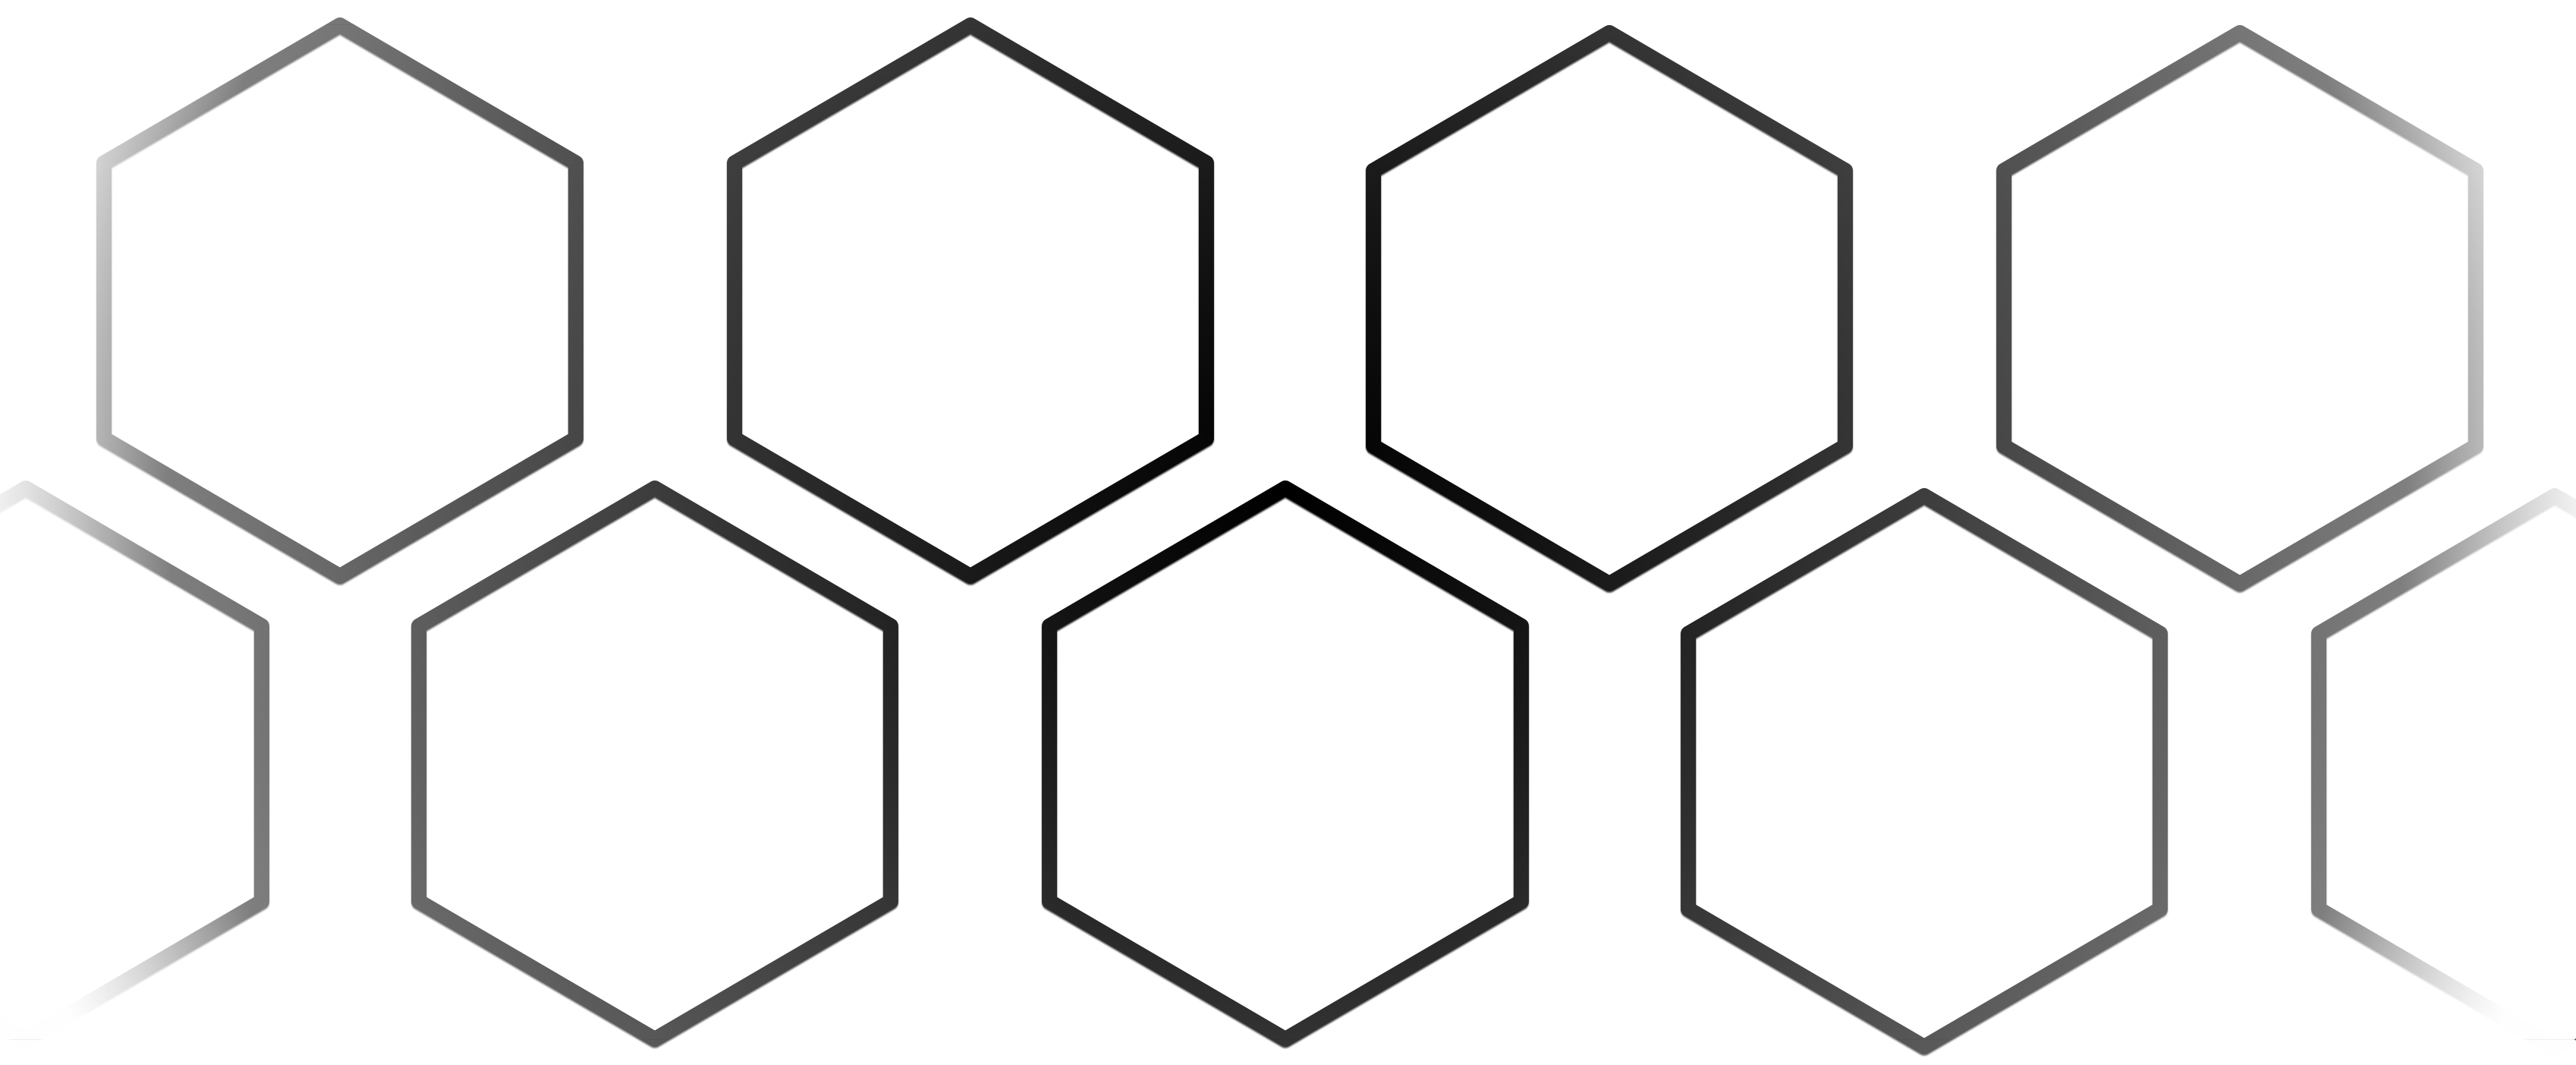
\includegraphics[width=\textwidth]{figures/complexity/hexRepeat.png}
    \vspace{5mm}
    
    \visible<3->{
    
\includegraphics[width=\textwidth]{figures/complexity/decompose.png}
    }
  \end{figure}
\end{column}

\begin{column}[T]{0.25\textwidth}
\centering
\vspace{5mm}

\visible<2->{
  \small{Complexity}
  \vspace{10mm}
}

\small{Tasks}

\visible<3->{
  \vspace{10mm}
  \small{Decomposition}
}

\end{column}
\end{columns}
\end{frame}


\begin{frame}[standout]
    What is the future of work?
\end{frame}

\begin{frame}{What is the future of work?}
    
\end{frame}



\begin{frame}{A Timeline of Crowdsourcing}
\visible<2->{
\begin{tikzpicture}
  [
    chronos={%
      % timeline width=50mm,
      timeline width=\textwidth,
      timeline height=2pt,
      start date={1880}-01-01,
      end date={1920}-01-01,
      events/.append style={font=\tiny},
      timeline year={font=\scriptsize},
      % timeline line={blue!40, shorten >=-20mm, -{Triangle Cap[length=20mm]}},
      only years,
      step years=5,
      timeline years=below,
      timeline marks,
    }
  ]

 \chronosevent {1888}{Match girls' strike~\cite{10.2307/3827491}} % (20pt)
 \chronosevent {1921}{\textcite{american1921problem}}
 \chronosevent {1904}{\textcite{richards1904anything}}
 \chronosevent {1896}{\textcite{taylor1896piece}}
 % \chronosevent{}
  \end{tikzpicture}
  \vspace{20mm}
  }

\begin{tikzpicture}
  [
    chronos={%
      % timeline width=50mm,
      timeline width=\textwidth,
      timeline height=2pt,
      start date={2006}-01-01,
      end date={2017}-01-01,
      events/.append style={font=\tiny},
      timeline year={font=\scriptsize},
      % timeline line={blue!40, shorten >=-20mm, -{Triangle Cap[length=20mm]}},
      only years,
      step years=1,
      timeline years=below,
      timeline marks,
    }
  ]

 % \chronosevent {1888}{Match girls' strike} % (20pt)
 % \chronosevent{}{\textcite{american1921problem}}
 % \eventcite{turkitLittle}
  \chronosevent{2008}{\textcite{Sheng:2008:GLI:1401890.1401965}}
  \chronosevent {2010}{\textcite{bernsteinSoylent,turkitLittle}}(-40pt)
  \chronosevent{2011}{\textcite{crowdForgeKittur}}
  \chronosevent{2013}{\textcite{lasecki2013chorus,chilton2013cascade,crowdworkFuture}}
 
 \chronosevent{2015}{\textcite{uberAlgorithm,dynamo}}(-30pt)
 % \chronosevent {2015}{\textcite{dynamo}}
 \chronosevent {2013}{\textcite{turkopticon}}
  \end{tikzpicture}



\end{frame}







\begin{frame}{Introduction}
  We hope to provide:
      \begin{itemize}
        \item A useful ontological lens for making sense of crowdsourcing and gig work (which we collectively call ``\textit{on--demand work}'') as a resurgence of \textit{piecework}.
        \item A method for making sense of contemporary phenomena through \textit{historical analysis}.
      \end{itemize}
\end{frame}

\end{document}